\documentclass{../notatki}
\geometry{margin=1cm, left=1cm, right=1cm, bottom=1cm, headsep=0.5cm}
\usepackage[fontsize=5pt]{scrextend}
\usepackage{multicol}
\fancyhead[C]{\href{https://github.com/TCA166/notes}{TCA166, Jager72}}
\fancyfoot{}

\makeatletter
\renewcommand
\section{\@startsection {section}{1}{\z@}%
  {-20pt plus -1pt minus -1pt}% space before
  {2pt plus 1pt minus 1pt}% space after
{\normalfont\large\bfseries}} % style
\makeatother

\title{Konspekt kompresja}

\begin{document}

\begin{multicols}{2}

  \section*{Wzory}

  \begin{multicols}{2}

    \begin{itemize}
      \item \textbf{Informacja:} $$I(x) = -\log_2 P(x)$$
      \item \textbf{Entropia:} $$H(X) = \sum P(x) \cdot I(x)$$
      \item \textbf{Śr. długość kodu:} $$L = \sum P_i \cdot l_i$$
      \item \textbf{Nierówność Krafta:} $$\sum 2^{-l_i} \leq 1$$
      \item \textbf{Wydajność:} $$r = \frac{1}{n} \log |\mathcal{C}|$$
    \end{itemize}

    \columnbreak

    \begin{itemize}
      \item \textbf{Hamming:} $d$ = liczba różnic
        \textbf{Wykrywanie:} $d - 1$, \textbf{Korekcja:} $\lfloor
        (d - 1)/2 \rfloor$
      \item \textbf{Wsp. informacji:} $\eta = k/n$
      \item \textbf{Kod doskonały:} $$\sum_{i=0}^{t} \binom{n}{i} \leq 2^{n-k}$$
      \item \textbf{Cykliczność:} \\ przesunięcie $\Rightarrow$ w kodzie
      \item \textbf{Wielomian $g(x)$:} $$g(x) \mid x^n + 1 \in \mathbb{Z}_2[x]$$
    \end{itemize}

  \end{multicols}

  \vspace{-2em}
  \textbf{Przykłady:}
  {\small
    $$
    I(1/2)=1, \quad H(\{1/2,1/2\})=1, \quad
    L=0.5\cdot1+0.5\cdot2=1.5, \quad \sum 2^{-l_i} = 0.75
    $$
  }

  \section*{Kod Huffmana}

  \begin{multicols}{2}

    \textbf{Algorytm:}
    \begin{itemize}
        \setlength{\itemsep}{1pt}
      \item Symbole $a_i$ z wagami ($P_i$ lub liczba wystąpień)
      \item Połącz 2 najmniejsze wagi $\rightarrow$ nowe drzewo
      \item Krawędzie: lewa = 0, prawa = 1
      \item Powtarzaj aż zostanie jedno drzewo
      \item Kody = ścieżki z korzenia
    \end{itemize}

    \columnbreak

    \textbf{Wariant dynamiczny:}
    \begin{itemize}
        \setlength{\itemsep}{1pt}
      \item Drzewo budowane w trakcie odczytu
      \item Nowe symbole $\Rightarrow$ użycie \texttt{NYT} (Not Yet Transmitted)
      \item Nowy symbol dodany do drzewa, reszta aktualizowana
      \item Znane symbole: kod z aktualnego drzewa
    \end{itemize}
    \textit{Kod prefiksowy, jednoznaczny, optymalny (min. $L$)}

  \end{multicols}

  \vspace{-2em}
  \section*{Kod Shannon-Fano}

  \textit{Kod prefiksowy, nie zawsze optymalny.}
  \begin{itemize}
    \item Dla $a_i$ z $p_i$: oblicz $l_i = \lceil -\log_2 p_i \rceil$
    \item Oblicz $w_j$: \quad $w_1 = 0$, \quad $w_j =
      \sum_{i=1}^{j-1} 2^{l_j - l_i}$
    \item Kod $a_j$: binarna postać $w_j$ dopełniona zerami z lewej
      do $l_j$ bitów
  \end{itemize}
  \textbf{Przykład:} $p = [0.5, 0.25, 0.25] \Rightarrow l = [1, 2, 2]$ \\
  $w = [0, 2, 3] \Rightarrow$ \quad kody: 0, 10, 11

  \section*{Kod Golomba/Rice}
  Dla liczby $n$ i parametru $M$:

  $$q = \lfloor \frac{n}{M} \rfloor, r = n \bmod M$$
  \textbf{Golomb:} kod = $q$ w unarnym + $r$ w binarnym (długość
  zależna od $M$)\\
  \textbf{Rice:} Golomb z $M = 2^k$ $\Rightarrow$ $r$ = $k$-bitowy binarny

  \section*{Kod Tunstalla}

  \textit{Kod nieprefiksowy, ale jednoznaczny przy stałej długości.}\\
  Kompresja bezstratna o stałej długości wyjściowej (kod: $n$ bitów):

  \begin{itemize}
    \item Dla alfabetu $a_i$ z $p_i$ budujemy drzewo od najczęstszych symboli.
    \item Rozwijaj liść $S$: twórz ciągi $Sa_1, \dots, Sa_m$ z wagą
      $P \cdot p_i$.
    \item Powtarzaj aż liczba liści (kodów) $= 2^n$.
    \item Kody to indeksy liści (słowa) $\Rightarrow$ długość kodu = $n$.
  \end{itemize}
  \textbf{Przykład:} $p(a)=0.6$, $p(b)=0.4$ $\Rightarrow$ start: $a$, $b$\\
  Rozwijaj $a$: $aa$, $ab$ itd. aż do np. 4 słów (dla $n=2$)

  \section*{Kodowanie Eliasa}

  Dla liczby całkowitej $x$, długości binarnej $n = \lfloor \log_2 x
  \rfloor + 1$:
  \begin{itemize}
    \item $\gamma(x) = 0^{n-1} \, (x)_2$
    \item $\delta(x) = \gamma(n) + (x)_2$ bez pierwszego bitu
    \item $\omega(x) = \omega(n-1) + (x)_2 + 0$ (rekurencja)
  \end{itemize}

  \textbf{Przykład:} $x = 9$, $(x)_2 = 1001$, $n = 4$ \\
  $\gamma(9) = 0001001$ \quad $\delta(9) = \gamma(4) + 001$ \\
  $\omega(9) = \omega(3) + 1001 + 0$
  \section*{Kodowanie Fibonacciego}

  \begin{itemize}
    \item Ciąg: $f_0 = f_1 = 1$, $f_n = f_{n-1} + f_{n-2}$ dla $n \geq 2$
    \item Reprezentacja liczby $x$: $x = \sum a_i f_i$, $a_i \in \{0,1\}$
    \item Warunek: brak dwóch jedynek obok siebie (Zeckendorfa)
    \item Na końcu dodajemy dodatkowe $1$ jako znacznik końca
  \end{itemize}
  \textbf{Przykład:} $x = 6$, $6 = 5 + 1 = f_4 + f_1$ $\Rightarrow$
  $100100$ + 1 = \texttt{1001001}

  \section*{Kodowanie arytmetyczne}
  \begin{multicols}{2}
    \textbf{Kodowanie:}
    \begin{itemize}
      \item $d = p - l$
      \item $l \gets l + d \cdot F(j)$
      \item $p \gets l + d \cdot F(j+1)$
    \end{itemize}
    \columnbreak
    \textbf{Dekodowanie:}
    \begin{itemize}
      \item $d = p - l$
      \item Znajdź $j$: $F(j) \leq \dfrac{x - l}{d} < F(j+1)$
      \item $l \gets l + d \cdot F(j)$
      \item $p \gets l + d \cdot F(j+1)$
    \end{itemize}
  \end{multicols}
  \textbf{Przykład:} $F = [0, 0.5, 1]$, dla ciągu \texttt{AB},
  $A=0$–$0.5$, $B=0.5$–$1$ \\
  Koniec przedziału: liczba z zakresu $(0.25, 0.75)$ reprezentuje
  słowo \texttt{AB}

  \section*{Kodowanie słownikowe}

  \begin{multicols}{3}
    \subsection*{LZ77}
    $$
    (o, l, k) = \mathcal{C}_{i - o} \dots \mathcal{C}_{i - o + l} \, k
    $$
    \footnotesize
    $o$ — przesunięcie, $l$ — długość, $k$ — nowy znak \\
    \textbf{Przykład:} \texttt{aabcaabc} \\
    (0,0,a), (0,0,a), (0,0,b), (0,0,c), (4,3,c)

    \vfill\null
    \columnbreak

    \subsection*{LZ78}
    \footnotesize
    Znajdź najdłuższy prefiks (lub $\epsilon$) \\
    Dodaj: prefiks + nowy znak \\
    Zakoduj: $(i,k)$ \\
    \textbf{Przykład:} \texttt{ababcbababaaaaaaa} \\
    (0,a), (0,b), (1,b), (0,c), (2,a), (4,a), (6,a), (7,a)

    \vfill\null
    \columnbreak

    \subsection*{LZW}
    \footnotesize
    Startowy słownik = alfabet \\
    Kodujemy indeksy ciągów $(i)$ \\
    Dodaj nowy ciąg gdy brak \\
    \textbf{Przykład:} \texttt{abababa} \\
    a (97), b (98), ab (256), ba (257), aba (258) \\
    Kody: 97, 98, 256, 257, 258
  \end{multicols}

  \vspace{-3em}

  \section*{BWT / bzip2}

  1. Dla słowa tworzymy wszystkie rotacje cykliczne.
  2. Sortujemy je leksykograficznie.
  3. Zapisujemy ostatnią kolumnę (BWT) i numer wiersza, gdzie
  znajduje się oryginalne słowo.
  4. Odwracanie: znając BWT i indeks, możemy odzyskać oryginalne słowo.

  \begin{center}
    \begin{tabular}{|c|c|}
      \hline
      e & h \\
      \hline
      \rowcolor{gray!25}
      h & o \\
      \hline
      ll & e \\
      \hline
      lo & l \\
      \hline
      o & l \\
      \hline
    \end{tabular}
    \quad
    \begin{tabular}{|c|c|c|c|c|}
      \hline
      \rowcolor{gray!25}
      0 & 1 & 2 & 3 & 4 \\
      \hline
      e & h & l & l & o \\
      \hline
      2 & 0 & 3 & 4 & 1 \\
      \hline
    \end{tabular}
  \end{center}

  \section*{Move-To-Front (MTF)}

  Transformacja zmniejszająca entropię (często po BWT).

  \begin{itemize}
    \item Start: tabela liter w porządku alfabetycznym
    \item Dla każdej litery: zapisz jej pozycję, przesuń ją na początek
  \end{itemize}

  \textbf{Przykład:} \texttt{hello}
  Alfabet: \texttt{[e, h, l, o]}
  \begin{tabular}{ll}
    h $\rightarrow$ 1 & tabela: [h, e, l, o] \\
    e $\rightarrow$ 1 & tabela: [e, h, l, o] \\
    l $\rightarrow$ 2 & tabela: [l, e, h, o] \\
    l $\rightarrow$ 0 & tabela: [l, e, h, o] \\
    o $\rightarrow$ 3 & tabela: [o, l, e, h]
  \end{tabular}

  \textbf{Wynik:} \texttt{11203}
  \section*{PPM}

  \begin{itemize}
    \item Dla symbolu sprawdzamy jego kontekst (max długość $n$).
    \item Przeglądamy konteksty: $n \to 0 \to -1$
    \item Dla $n \geq 0$: zliczamy wystąpienia; dla $-1$: tylko obecność.
    \item Budujemy model prawdopodobieństw — np. do Huffmana.
  \end{itemize}
  \textbf{!:} szukaj symbolu w najdłuższym kontekście. Jeśli nie ma –
  wypisz ESC i przejdź do krótszego.
  \vspace{-1.5em}

  \begin{center}
    \resizebox{0.9\linewidth}{!}{
      \begin{tabular}{|c|}
        \hline
        Symbol \\ \hline
        t \\ h \\ i \\ s \\ - \\
        \hline
      \end{tabular}
      \quad
      \begin{tabular}{|c|c|}
        \hline
        Symbol & Licznik \\ \hline
        ESC & 1 \\ t & 1 \\ h & 1 \\ i & 1 \\ s & 2 \\ - & 1 \\
        \hline
      \end{tabular}
      \quad
      \begin{tabular}{|c|c|c|}
        \hline
        Kontekst & Symbol & Licznik \\ \hline
        t & ESC & 1 \\ & h & 1 \\ \hline
        h & ESC & 1 \\ & i & 1 \\ \hline
        i & ESC & 1 \\ & s & 2 \\ \hline
        s & ESC & 1 \\ & - & 1 \\ \hline
        - & ESC & 1 \\ & i & 1 \\
        \hline
      \end{tabular}
      \quad
      \begin{tabular}{|c|c|c|}
        \hline
        Kontekst & Symbol & Licznik \\ \hline
        th & ESC & 1 \\ & i & 1 \\ \hline
        hi & ESC & 1 \\ & s & 1 \\ \hline
        is & ESC & 1 \\ & - & 1 \\ \hline
        s- & ESC & 1 \\ & i & 1 \\ \hline
        -i & ESC & 1 \\ & s & 1 \\
        \hline
      \end{tabular}
    }
  \end{center}
  \vspace{-1em}

  \section*{Kody Hamminga}

  \begin{itemize}
    \item Długość kodu: $n = 2^m - 1$, dane: $k = n - m$
    \item Macierz parzystości $H$: kolumny = binarne zapisy $1, \dots, n$
  \end{itemize}
  \vspace{-0.5em}
  \[
    H_H(3) =
    \begin{bmatrix}
      0 & 0 & 0 & 1 & 1 & 1 & 1 \\
      0 & 1 & 1 & 0 & 0 & 1 & 1 \\
      1 & 0 & 1 & 0 & 1 & 0 & 1
    \end{bmatrix}
  \]

  \begin{itemize}
    \item Macierz generująca $G$: $[I_k \mid P]$, gdzie $P$ pochodzi z $H$
  \end{itemize}
  \vspace{-0.5em}
  \[
    G_H(3) =
    \begin{bmatrix}
      1 & 0 & 0 & 0 \\
      0 & 1 & 0 & 0 \\
      0 & 0 & 1 & 0 \\
      0 & 0 & 0 & 1 \\
      0 & 1 & 1 & 1 \\
      1 & 0 & 1 & 1 \\
      1 & 1 & 0 & 1
    \end{bmatrix}
  \]

  \textbf{Rozszerzony kod Hamminga:} dodany bit parzystości – długość $n + 1$
  \textbf{Cykliczny kod Hamminga:} generowany przez $g(x)$, który
  dzieli $x^n + 1$ w $\mathbb{Z}_2[x]$
  \textbf{Kod Hamminga (7,4)} jest kodem doskonałym dla $d = 3$

  \begin{multicols}{2}

    \begin{center}
      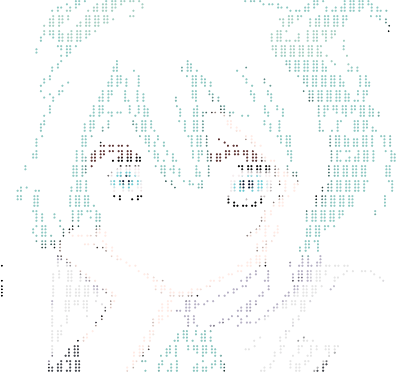
\includegraphics[width=17em]{emotionalSupportMiku.png} % Adjust
      % width as needed

      \begin{center}
        Fig. 1: Exam Emotional Support System\\
        \textbf{Hatsune przypomina:} Nie da się skompresować
        wszystkich możliwych słów — zbiór skompresowanych musi być
        mniejszy => nie istnieje bijekcja.

      \end{center}
    \end{center}
    \columnbreak
    \begin{quote}
      \textbf{Lew:} Twoja pewność siebie jest jak kod Huffmana —
      konkretna i skuteczna.

      \textbf{Ryby:} Chaos w danych? Nie szkodzi — PPM poradzi sobie
      nawet z tobą.

      \textbf{Wodnik:} BWT to twoja dusza — nieoczywista, ale piękna
      w dekodowaniu.

      \textbf{Koziorożec:} Twoja determinacja przypomina kod Hamminga
      — wykrywa, poprawia i nie odpuszcza.
    \end{quote}

  \end{multicols}

  \begin{center}
    \fbox{\phantom{\rule{1em}{1em}}}
    \fbox{\phantom{\rule{1em}{1em}}}
    \fbox{\phantom{\rule{1em}{1em}}}
    \fbox{\phantom{\rule{1em}{1em}}}
    \fbox{\phantom{\rule{1em}{1em}}}
  \end{center}
  \vspace{-0.8em}
  \begin{center}
    \footnotesize Fig. 2: Zakreśl, jeśli: \textit{Błąd w
    obliczeniach? Brak pomysłu? Nie rozumiesz pytania?}
  \end{center}
  \begin{center}
    \vspace{-0.5em}
    \textit{“Wszystko da się skompresować. Poza czasem na egzaminie.”} \\
    -- autor nieznany, ale na pewno sfrustrowany
  \end{center}
\end{multicols}

\end{document}